\documentclass[12pt, letterpaper, twoside]{article}
\usepackage[utf8]{inputenc}
\usepackage[a4paper]{geometry}
\usepackage{array}
\usepackage{booktabs} % For prettier tables
\usepackage{multirow}
\usepackage{multicol}
\usepackage{ragged2e}
\usepackage{xcolor}
\usepackage{gensymb}
\usepackage{fullpage}
\usepackage{hyperref}
\usepackage{amsmath}
\usepackage{scrextend}
\usepackage{graphicx}
\usepackage{tikz}
\usepackage{enumitem}

\graphicspath{ {./bilder/} }
\title{Vecka 19, Repetition betingad sannolikhet}
\author{Simon Freiermuth \\ \href{mailto:simon@freiermuth.org}{simon@freiermuth.org}}
\date{6 Maj, 2020}

\begin{document}

%\begin{titlepage}
\maketitle
%\end{titlepage}

\begin{flushleft}
\large\textbf{Betingad sannolikhet med venndiagramm:}\\
$ U $ är allt, det representerar alla objekt, i den här uppgiften är det alla 25 studenter.
Anta att vi har två händelser $ A $ och $ B $.\\
$ A|B $ Används för att representera att $ A $ händer givet att $ B $ har hänt. Dvs $ U $
har reducerats till $ B $.\\
Om man föreställer sig ett Universum som innehåller solsystemet $ B $, så när man säger att
"$ B $ händer" menar man att fokus reduceras till Solsystemet $ B $, och allt annat fösvinner.
Det nya $ U $ är nu samma som $ B $. Om man då tittar på $ A $ ser man bara den delen av $ A $
som är innuti $ B $.

\hfill

    \begin{tikzpicture}[fill=gray]
        % left hand
%        \scope
%            \clip (-2,-2) rectangle (2,2)
%                  (1,0) circle (1);
%            \fill (0,0) circle (1);
%        \endscope
%        % right hand
%        \scope
%            \clip (-2,-2) rectangle (2,2)
%                  (0,0) circle (1);
%            \fill (1,0) circle (1);
%        \endscope
        % outline
        \draw (-2,0)   circle    (4) (-2,4)  node [text=black,above] {$A$}
              (2,0)    circle    (4) (2,4)   node [text=black,above] {$B$}
              (-7,-5)  rectangle (7,5)       node [text=black,above] {$H$};
    \end{tikzpicture}



\hfill

\begin{enumerate}[label=\textbf{\arabic* .}]
%%%%%%%%%%%%%%%%%%%%%%%%%%%%%%%%%%%%%%%%%%%%%%%%%%%%%%%%%%%%%%%%%%%%%%%%%%%%%%%%%%%%%%%%%%%%%%
%   1.
%%%%%%%%%%%%%%%%%%%%%%%%%%%%%%%%%%%%%%%%%%%%%%%%%%%%%%%%%%%%%%%%%%%%%%%%%%%%%%%%%%%%%%%%%%%%%%
    \item
    I en grupp av 50 elever studerar 40 matte och 32 fysik.\\
    Alla studerar minst ett av ämnena.
    \begin{enumerate}[label=\textbf{\alph*)}]
        \item
        Med hjälp av ett venndiagramm, beräkna antalet elever som studerar båda ämnena.

        \textcolor{red}{
            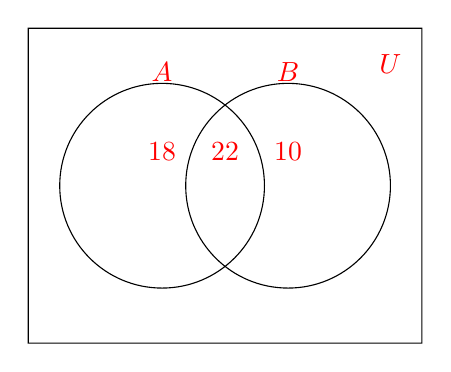
\begin{tikzpicture}[fill=red]
                \draw (-0.3,0) circle    (1.3) (-0.3,1.2) node [text=red,above] {$A$}
                (-0.3,0.2) node [text=red,above] {$18$}
                (0.5,0.2) node [text=red,above] {$22$}
                    (1.3,0)  circle    (1.3)
                    (1.3,1.2)  node [text=red,above] {$B$}
                    (1.3,0.2)  node [text=red,above] {$10$}
                    (-2,-2)  rectangle (3,2) (2.6,1.3)  node [text=red,above] {$U$};
            \end{tikzpicture} \\
            $$ n(A) = 40 \rightarrow\ Matte $$\\
            $$ n(B) = 32 \rightarrow\ Fysik $$\\
            $$ n(U) = 50 $$\\
            \hfill \\
            $$ n(A \cup B) = n(U) $$\\
            $$ n(A\cap B) = n(A) + n(B) - n(A \cup B) $$\\
            $$ n(A \cap B) = 40 + 32 - 50 = 22 $$
        }

        \hfill

        \item
        Om en elev väljs ut på måfå, hur stor är sannolikheten att:

        \begin{enumerate}[label=\textbf{\roman*.}]
            \item
            eleven studerar matte men inte fysik?

            \textcolor{red}{
                $$ p(A \cap ^- B) = \frac{n(A) - n(A \cap B)}{n(U)} $$
                $$ p(A \cap ^- B) = \frac{40 - 22}{50} = 0.36 = 36\% $$
            }

            \hfill

            \item
            eleven studerar fysik givet att eleven studerar matte?

            \textcolor{red}{
                $$ p(B|A) = \frac{p(B \cap A)}{p(A)} $$
                $$ p(B|A) = \frac{22}{40} = 0.55 = 55\% $$
            }
        \end{enumerate}
    \end{enumerate}


    \item
    I en klass med 40 elever har 23 mörkt hår, 18 har bruna ögon och 26 har minst en av det två.\\
    Om en elev väljs ut på måfå, hur stor är sannolikheten att eleven:

       \textcolor{red}{
            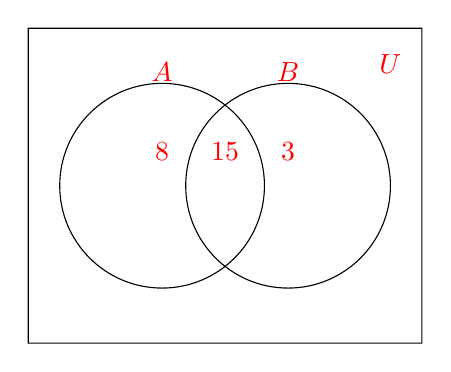
\begin{tikzpicture}[fill=red]
                \draw (-0.3,0) circle    (1.3) (-0.3,1.2) node [text=red,above] {$A$}
                (-0.3,0.2) node [text=red,above] {$8$}
                (0.5,0.2) node [text=red,above] {$15$}
                    (1.3,0)    circle    (1.3)
                    (1.3,1.2)  node [text=red,above] {$B$}
                    (1.3,0.2)  node [text=red,above] {$3$}
                    (-2,-2)    rectangle (3,2) (2.6,1.3)  node [text=red,above] {$U$};
            \end{tikzpicture}\\
            $ n(A) = 23 \rightarrow $ mörkt hår\\
            $ n(B) = 18 \rightarrow $ bruna ögon\\
            $ n(U) = 40 $\\
            $ n(A \cup B) = 26 $\\
        }

    \begin{enumerate}[label=\textbf{\alph*)}]
        \item
        har mörkt hår och bruna ögon?\\
        \textcolor{red}{
            $$ n(A\cap B) = n(A) + n(B) - n(A \cup B) $$
            $$ n(A\cap B) = 23 + 18 - 26 = 15 $$
            $$ p(A\cap B) = \frac{n(A\cap B)}{n(U)} $$
            $$ p(A\cap B) = \frac{15}{40} = 0.375 = 37.5\% $$
            Alternativt kan man baka ihop formlerna så här:
            $$ p(A\cap B) = \frac{n(A) + n(B) - n(A \cup B)}{n(U)} $$
            Det går snabbare om man kan göra allt i ett steg. (det är mer elegant också)
        }

        \item
        varken mörkt hår, eller bruna ögon?

        \textcolor{red}{
            $$ n(^-A) = n(U) - n(A) $$
            $$ n(^-A) = 40 - 23 = 17 $$
            $$ n(^-B) = 40 - 18 = 22 $$
            $$ n(^-A \cap ^-B) = n(U) - n(A \cup B) $$
            $$ n(^-A \cap ^-B) = 40 - 26 = 14 $$
            $$ p(^-A \cap ^-B) = \frac{n(^-A \cap ^-B)}{n(U)} $$
            $$ p(^-A \cap ^-B) = \frac{14}{40} = 0.35 = 35\% $$
        }

        \item
        har mörkt hår, men inga bruna ögon?

        \textcolor{red}{
            $$ p(A \cap ^-B) = \frac{n(A \cup B) - n(B)}{n(U)}  $$
            $$ p(A \cap ^-B) = \frac{26 - 18}{40} = 0.2 = 20\% $$
        }

        \item
        har bruna ögon, givet att eleven har mörkt hår?
    \textcolor{red}{
                $$ p(A|B) = \frac{p(B \cap A)}{p(B)} $$
                $$ p(A|B) = \frac{15}{18} = 0.83 = 83\% $$
            }
    \end{enumerate}
\end{enumerate}

\end{flushleft}
\end{document}
